\documentclass[../main/main.tex]{subfiles}

\newdate{date}{23}{11}{2020}

% \begin{figure}[h!]
% \centering
% \includegraphics[page=6,width=0.8\textwidth]{../lessons/pdf_file/19_lecture.pdf}
% \end{figure}

%\displaydate{date}. Compiled:  \today. Alice.

\begin{document}

\pagestyle{plain}

\section{Lecture 19}


\subsubsection*{Slide 1}

\begin{minipage}[]{0.5\linewidth}
\centering
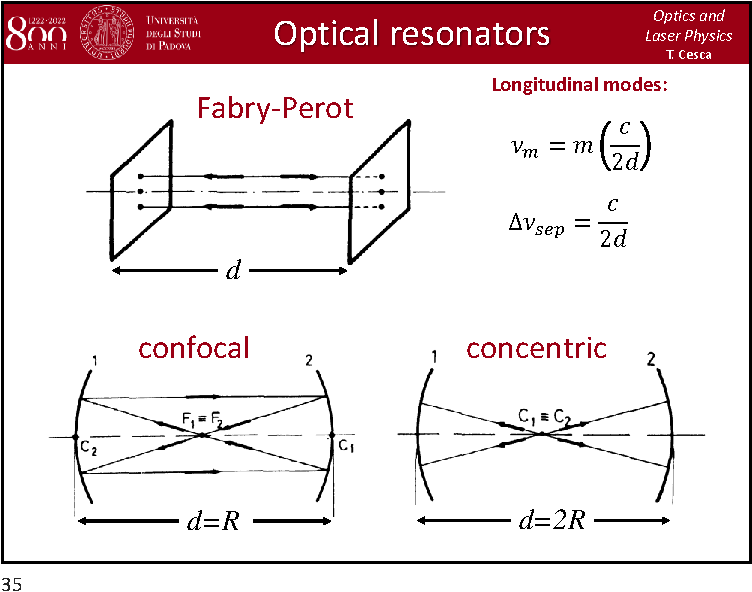
\includegraphics[page=1,width=1\textwidth]{../lessons/pdf_file/19_lecture.pdf}
\end{minipage}
\hspace{0.3cm}\vspace{0.3cm}
\begin{minipage}[c]{0.47\linewidth}

The Fabry-Perot is not the most practical one, because of the allineation of the two mirrors.

Another possibility is the \textbf{confocal cavity} composed by two spherical mirrors with the same \emph{focal point}, where the distance between them is equal to the radius of curvature. This means that the focal point is a the same position.

In a \textbf{concentric cavity} the center of curvature of these spherical mirror is in the same position.

\end{minipage}

\subsubsection*{Slide 2}

\begin{minipage}[]{0.5\linewidth}
\centering
\includegraphics[page=2,width=1\textwidth]{../lessons/pdf_file/19_lecture.pdf}
\end{minipage}
\hspace{0.3cm}\vspace{0.3cm}
\begin{minipage}[c]{0.47\linewidth}

One example of asymmetric configuration is the \textbf{emifocal cavity}, the focal point is at the position of the plane mirror.

From now \( R \) is indicating the radius of curvature of the spherical mirror!

We have also an \textbf{emiconcentric cavity} in which the spherical mirror and the plane mirror are at distance \( R \) such that the plane mirror is in the center of the spherical mirror.

\end{minipage}

\subsubsection*{Slide 3}

\begin{minipage}[]{0.5\linewidth}
\centering
\includegraphics[page=3,width=1\textwidth]{../lessons/pdf_file/19_lecture.pdf}
\end{minipage}
\hspace{0.3cm}\vspace{0.3cm}
\begin{minipage}[c]{0.47\linewidth}

We can have more complex configurations as \textbf{ring resonators}. In this case we should consider the effective perimeter of the cavity.

\end{minipage}

\newpage

\subsubsection*{Slide 4}

\begin{minipage}[]{0.5\linewidth}
\centering
\includegraphics[page=4,width=1\textwidth]{../lessons/pdf_file/19_lecture.pdf}
\end{minipage}
\hspace{0.3cm}\vspace{0.3cm}
\begin{minipage}[c]{0.47\linewidth}

For \textbf{unstable resonators} means that the photons after a certain number of passes leave the cavity. In any optical cavity the photon go back and forth thousand of times, so with an unstable resonator you can have the photons leaving the cavity. However for unstable resonator is possible to realize very large beams with a hole in the middle visible when you see the spot near the outcoupling mirror.

Another example of unstable resonator is the \textbf{confocal telescopic resonator}.


\end{minipage}

\subsubsection*{Slide 5}

\begin{minipage}[]{0.5\linewidth}
\centering
\includegraphics[page=5,width=1\textwidth]{../lessons/pdf_file/19_lecture.pdf}
\end{minipage}
\hspace{0.3cm}\vspace{0.3cm}
\begin{minipage}[c]{0.47\linewidth}

In order to establish if a cavity is stable or unstable, its important to remember some concepts of \emph{geometrical optics}.

Firstly, we should define the \textbf{sign convention}.  We consider always light coming from left to right. We will work always with spherical surfaces with radius of curvature \( R \) (we can approximate any surface as a sphere locally).
The two media between the spherical surfaces have different refractive index.

We will work with the \textbf{central optical system}: all the optical elements are aligned in the same optical axis.

In the vertex the surface intercepts the optical axis. If the surface is convex from the light coming from left, the radius is positive.

Object: \( p \) and \( y \).

Image: \( q \) and \( y' \).


\end{minipage}

\subsubsection*{Slide 6}

\begin{minipage}[]{0.5\linewidth}
\centering
\includegraphics[page=6,width=1\textwidth]{../lessons/pdf_file/19_lecture.pdf}
\end{minipage}
\hspace{0.3cm}\vspace{0.3cm}
\begin{minipage}[c]{0.47\linewidth}

All the expression that we are writing are in the \textbf{paraxial approximation}: all the angles are small that you can approximate the sin of the angle and the tangent with the angle itself (so the distance from the optical axis are so small).

\end{minipage}

\newpage

\subsubsection*{Slide 7}

\begin{minipage}[]{0.5\linewidth}
\centering
\includegraphics[page=7,width=1\textwidth]{../lessons/pdf_file/19_lecture.pdf}
\end{minipage}
\hspace{0.3cm}\vspace{0.3cm}
\begin{minipage}[c]{0.47\linewidth}

A thin lens is a block of material with two spherical surfaces. It separate two media with different refractive indexes.

A thin lens is when \( s \) is so small wrt other distances that can be neglected.

In this case from the equation of the \textbf{spherical diopter} we can write the \textbf{thin lens equation}. We are assuming \( n_1 = n_3 \).


\( f \) is the \textbf{focal length of the lens}.
We can determine it by the \textbf{Lens-maker's equation}.

All the quantities have a sign! Also \( f \) can have one!

Moreover, the focal length of most of the situation is given ever when \( n_1 = n_3 \)!

\end{minipage}

\subsubsection*{Slide 8}

\begin{minipage}[]{0.5\linewidth}
\centering
\includegraphics[page=8,width=1\textwidth]{../lessons/pdf_file/19_lecture.pdf}
\end{minipage}
\hspace{0.3cm}\vspace{0.3cm}
\begin{minipage}[c]{0.47\linewidth}

If the focal length is positive, the lens is a \textbf{converging lens}.

If the focal length is negative, the lens is a \textbf{diverging lens}.

\end{minipage}

\subsubsection*{Slide 9}

\begin{minipage}[]{0.5\linewidth}
\centering
\includegraphics[page=9,width=1\textwidth]{../lessons/pdf_file/19_lecture.pdf}
\end{minipage}
\hspace{0.3cm}\vspace{0.3cm}
\begin{minipage}[c]{0.47\linewidth}

Let us imagine to have a \textbf{thin lens}. When the tips of the arrow are in this way, we have a \textbf{converging} thin lens.

We have the \textbf{forward focal point} and the \textbf{backward focal point}.

There is a ray parallel to the optical axis (it means \( p = \infty  \)). From the lens equation we have that \( q = f \). So the image will be formed at the focal point of the lens!

Let us consider an object placed at \( P_1 \), we have that \( p=f \). We obtain \( q = \infty  \). The ray is coming parallel to the optical axis!


\end{minipage}

\subsubsection*{Slide 10}

\begin{minipage}[]{0.5\linewidth}
\centering
\includegraphics[page=10,width=1\textwidth]{../lessons/pdf_file/19_lecture.pdf}
\end{minipage}
\hspace{0.3cm}\vspace{0.3cm}
\begin{minipage}[c]{0.47\linewidth}

Graphical tool to obtain the position of an image formed when the rays of light coming from an object imping on a thin lens.

We can get both quality and quantitative informations if we do the drawing in scale.

Three specific rays are enough to determine the position where the image is forms both for converging and diverging lenses.


\end{minipage}

\subsubsection*{Slide 11}

\begin{minipage}[]{0.5\linewidth}
\centering
\includegraphics[page=11,width=1\textwidth]{../lessons/pdf_file/19_lecture.pdf}
\end{minipage}
\hspace{0.3cm}\vspace{0.3cm}
\begin{minipage}[c]{0.47\linewidth}

We have a virtual image in the second case. There is no energy! It is just virtual.. it is formed by the extension of the rays on the back.

So the converging lens behave as before the focal point. Otherwise it behaves as diverging.

Instead, the diverging lens is always behaving as diverging. You always have the formation of virtual images.

\end{minipage}

\subsubsection*{Slide 12}

\begin{minipage}[]{0.5\linewidth}
\centering
\includegraphics[page=12,width=1\textwidth]{../lessons/pdf_file/19_lecture.pdf}
\end{minipage}
\hspace{0.3cm}\vspace{0.3cm}
\begin{minipage}[c]{0.47\linewidth}

We can calculate the \textbf{magnification}: the size of the image wrt the size of the object.

\end{minipage}

\subsubsection*{Slide 13}

\begin{minipage}[]{0.5\linewidth}
\centering
\includegraphics[page=13,width=1\textwidth]{../lessons/pdf_file/19_lecture.pdf}
\end{minipage}
\hspace{0.3cm}\vspace{0.3cm}
\begin{minipage}[c]{0.47\linewidth}

It is possible to write the equivalent of the thin lens equation also for a spherical mirror.

\end{minipage}

\subsubsection*{Slide 14}

\begin{minipage}[]{0.5\linewidth}
\centering
\includegraphics[page=14,width=1\textwidth]{../lessons/pdf_file/19_lecture.pdf}
\end{minipage}
\hspace{0.3cm}\vspace{0.3cm}
\begin{minipage}[c]{0.47\linewidth}

We can do ray tracing also in this case.

\end{minipage}

\subsubsection*{Slide 15}

\begin{minipage}[]{0.5\linewidth}
\centering
\includegraphics[page=15,width=1\textwidth]{../lessons/pdf_file/19_lecture.pdf}
\end{minipage}
\hspace{0.3cm}\vspace{0.3cm}
\begin{minipage}[c]{0.47\linewidth}

Try to do these exercises!

\end{minipage}

\subsubsection*{Slide 16}

\begin{minipage}[]{0.5\linewidth}
\centering
\includegraphics[page=16,width=1\textwidth]{../lessons/pdf_file/19_lecture.pdf}
\end{minipage}
\hspace{0.3cm}\vspace{0.3cm}
\begin{minipage}[c]{0.47\linewidth}

Let us introduce the tool of \textbf{ABCD matrices}.

\( x \) is the hight wrt the optical axis and \( \theta  \) is the inclination. These two elements form a \textbf{ray vector}.

Moreover, for any optical system we can introduce a matrix.
The order of the matrix is important: the first matrix on the right is the first optical element the beam encounters.


\end{minipage}

\subsubsection*{Slide 17}

\begin{minipage}[]{0.5\linewidth}
\centering
\includegraphics[page=17,width=1\textwidth]{../lessons/pdf_file/19_lecture.pdf}
\end{minipage}
\hspace{0.3cm}\vspace{0.3cm}
\begin{minipage}[c]{0.47\linewidth}

Let us consider the first simpler situation. \textbf{Free-space propagation} means the propagation inside the same medium (not in vacuum!). So, there is no change in refractive index, independent on its value. So light beam is not deflected by anything.

We will work with the paraxial approximation.

\end{minipage}

\subsubsection*{Slide 18}

\begin{minipage}[]{0.5\linewidth}
\centering
\includegraphics[page=18,width=1\textwidth]{../lessons/pdf_file/19_lecture.pdf}
\end{minipage}
\hspace{0.3cm}\vspace{0.3cm}
\begin{minipage}[c]{0.47\linewidth}

Let us consider a \textbf{plane diopter}: plane surface separating two media with different refractive index.

\end{minipage}

\subsubsection*{Slide 19}

\begin{minipage}[]{0.5\linewidth}
\centering
\includegraphics[page=19,width=1\textwidth]{../lessons/pdf_file/19_lecture.pdf}
\end{minipage}
\hspace{0.3cm}\vspace{0.3cm}
\begin{minipage}[c]{0.47\linewidth}

Let us consider a \textbf{spherical diopter} with radius of curvature \( R \). It separates the two media with different refractive index.

\end{minipage}

\subsubsection*{Slide 20}

\begin{minipage}[]{0.5\linewidth}
\centering
\includegraphics[page=20,width=1\textwidth]{../lessons/pdf_file/19_lecture.pdf}
\end{minipage}
\hspace{0.3cm}\vspace{0.3cm}
\begin{minipage}[c]{0.47\linewidth}

These are the most relevant matrices for most of the optical elements.

\end{minipage}

\subsubsection*{Slide 21}

\begin{minipage}[]{0.5\linewidth}
\centering
\includegraphics[page=21,width=1\textwidth]{../lessons/pdf_file/19_lecture.pdf}
\end{minipage}
\hspace{0.3cm}\vspace{0.3cm}
\begin{minipage}[c]{0.47\linewidth}

Let us compute the ABCD matrix for a \textbf{thin lens}. We can compute the matrix as the combination of the matrices of two spherical dipters with two different radii.

\end{minipage}

\subsubsection*{Slide 22}

\begin{minipage}[]{0.5\linewidth}
\centering
\includegraphics[page=22,width=1\textwidth]{../lessons/pdf_file/19_lecture.pdf}
\end{minipage}
\hspace{0.3cm}\vspace{0.3cm}
\begin{minipage}[c]{0.47\linewidth}

In the same case we can solve the situation of two thin lenses.
We can define an \textbf{effective focal length}.


\end{minipage}


\end{document}
